\chapter{Structures discrètes sur l'Internet}

\section{Ressources}
Ressource pour cette partie du cours :\\
Networks, Crowds, and Markets: Reasoning About a Highly Connected World, by David Easley and Jon Kleinberg

\begin{itemize}
\item Chapitre 1-5 (Graphe = modèle des réseaux) définitions, concepts (liens forts et faibles), contexte des réseaux, relations positives et négatives
\item Chapitre 13 (Structure du web)
\item Chapitre 14 (Analyse des liens sur le web)
\item Chapitre 18 (Lois de puissances)
\item Chapitre 20 (Les phénomènes de petit monde)
\end{itemize}

\section{Exemple et analyse de graphes}
Voici quelques commentaires réalisés sur les figures du $1^{er}$ chapitre :

\begin{itemize}

	\item \textbf{Figure 1.1} (ci-dessous : Figure \ref{karate} Illustration des relations amicales entre 34 personnes dans un club de karaté.
Chaque nœud représente une personne et chaque lien, un lien d'amitié entre ces personnes.
On constate que tout le monde n'est pas ami avec tout le monde. Grâce à cette structure, on peut déduire certaines choses, par exemple : deux personnes ont beaucoup de liens d'amitié avec d'autres personnes, mais pas entre eux.

\begin{center}
\begin{figure}[!ht]
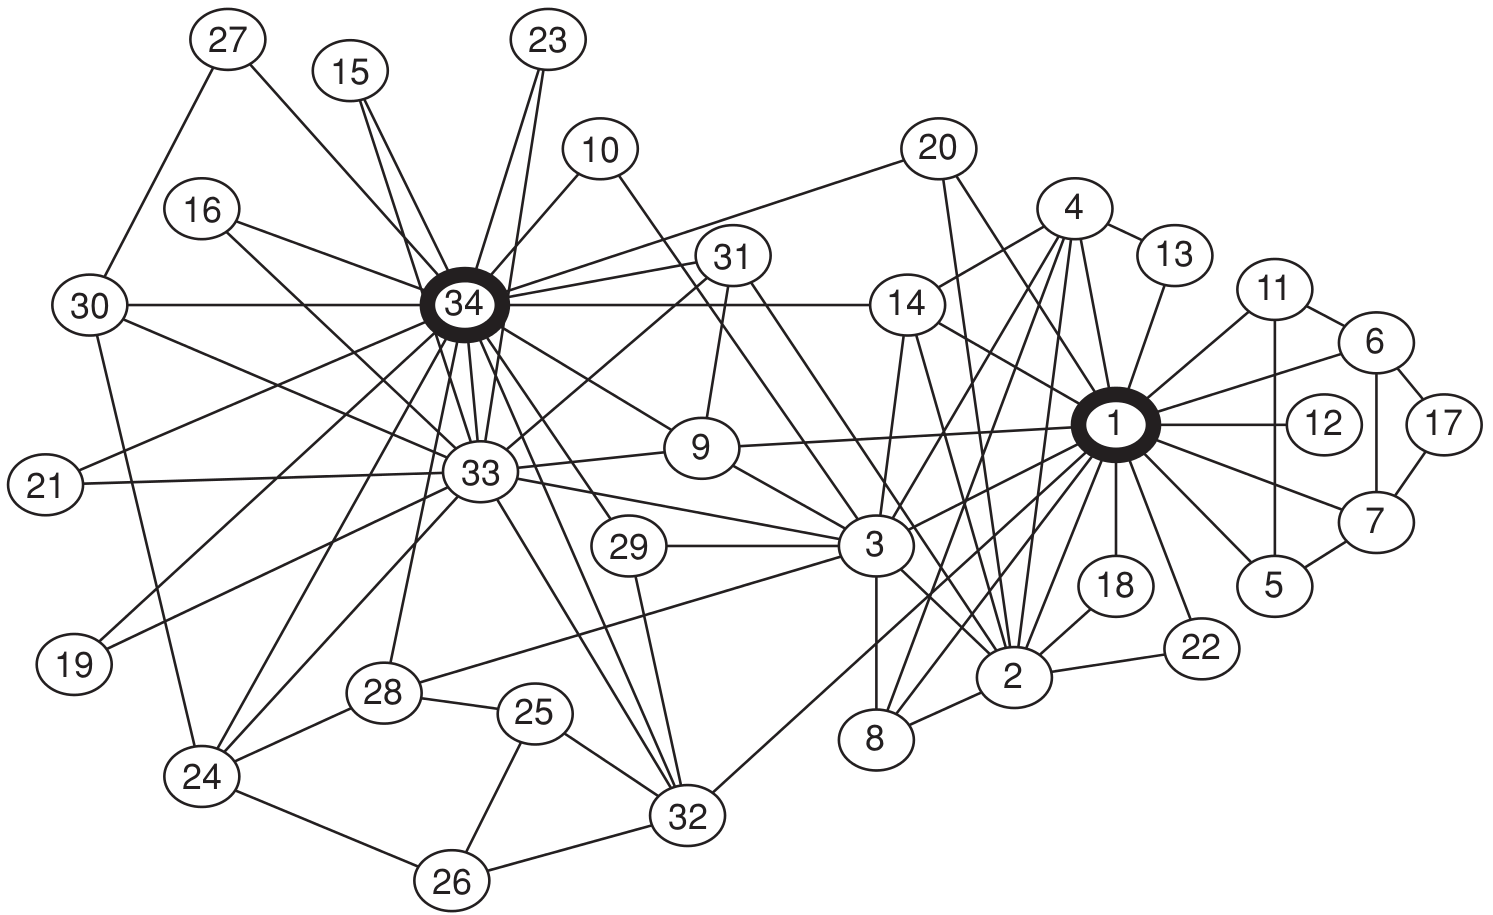
\includegraphics[width=0.9\linewidth]{images/17_karate_club.png}
\label{karate}
\caption{Relations amicales dans un club de karaté}
\end{figure}
\end{center}

	\item \textbf{Figure 1.2} Des employés dans un laboratoire de recherche (nœud) ont des liens entre eux :
Lignes claires = communication e-mail.
Lignes foncées = hiérarchie, organisation du laboratoire.
On voit que la communication entre les gens suit relativement bien la structure hiérarchique, mais pas complètement. On peut voir comment les gens collaborent, leurs degrés de collaboration, etc.

\begin{figure}[!ht]
\centering
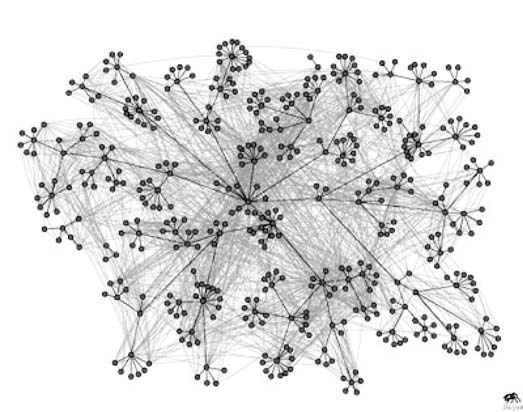
\includegraphics[width=0.8\linewidth]{images/social_networks_based_on_communication_and_interaction.png}
\end{figure}

	\item \textbf{Figure 1.3} On constate que dans cette illustration, il y a beaucoup plus de nœuds. Chaque nœud est une institution financière (banque par exemple). Les liens représente des relations entre les banques, c'est à dire des prêts faits par une banque à une autre. Le graphe est connexe (il y a des chemins entre toutes les banques). Le centre est très dense, ça montre une faiblesse du système financier : si une banque dans le centre fait faillite par exemple, toutes les autres banques liées à elle sont également mises en danger . Donc si le noyau central est trop grand, c'est une faiblesse. En regardant cette structure, on peut trouver les faiblesses et les comprendre. Ça peut être très important.
\begin{figure}[!ht]
\centering
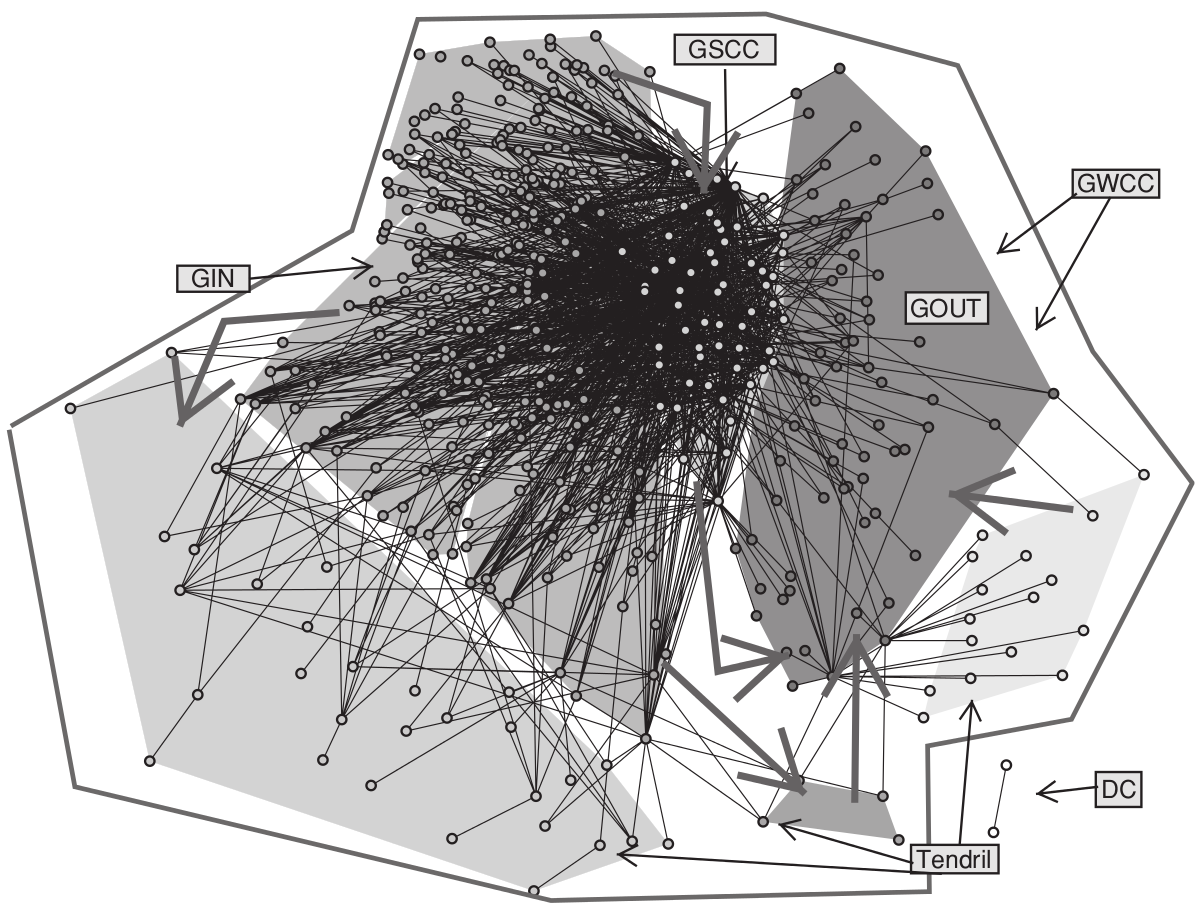
\includegraphics[width=0.8\linewidth]{images/reseaux_prets_entre_banques.png}
\end{figure}

	\item \textbf{Figure 1.4} Un nœud représente un blog politique et un lien, une référence vers un autre blog. Nous avons deux partis qui représentent chacun un noyau : les démocrates et les républicains. On constate qu'il y a moins de connexions entre les deux noyaux qu'à l'intérieur de ceux-ci. On peut visualiser cette structure et se poser des questions : est-ce que cette absence de contact entre les deux factions d'un monde bipolaire est un problème ?
\end{itemize}

\begin{figure}[!ht]
\centering
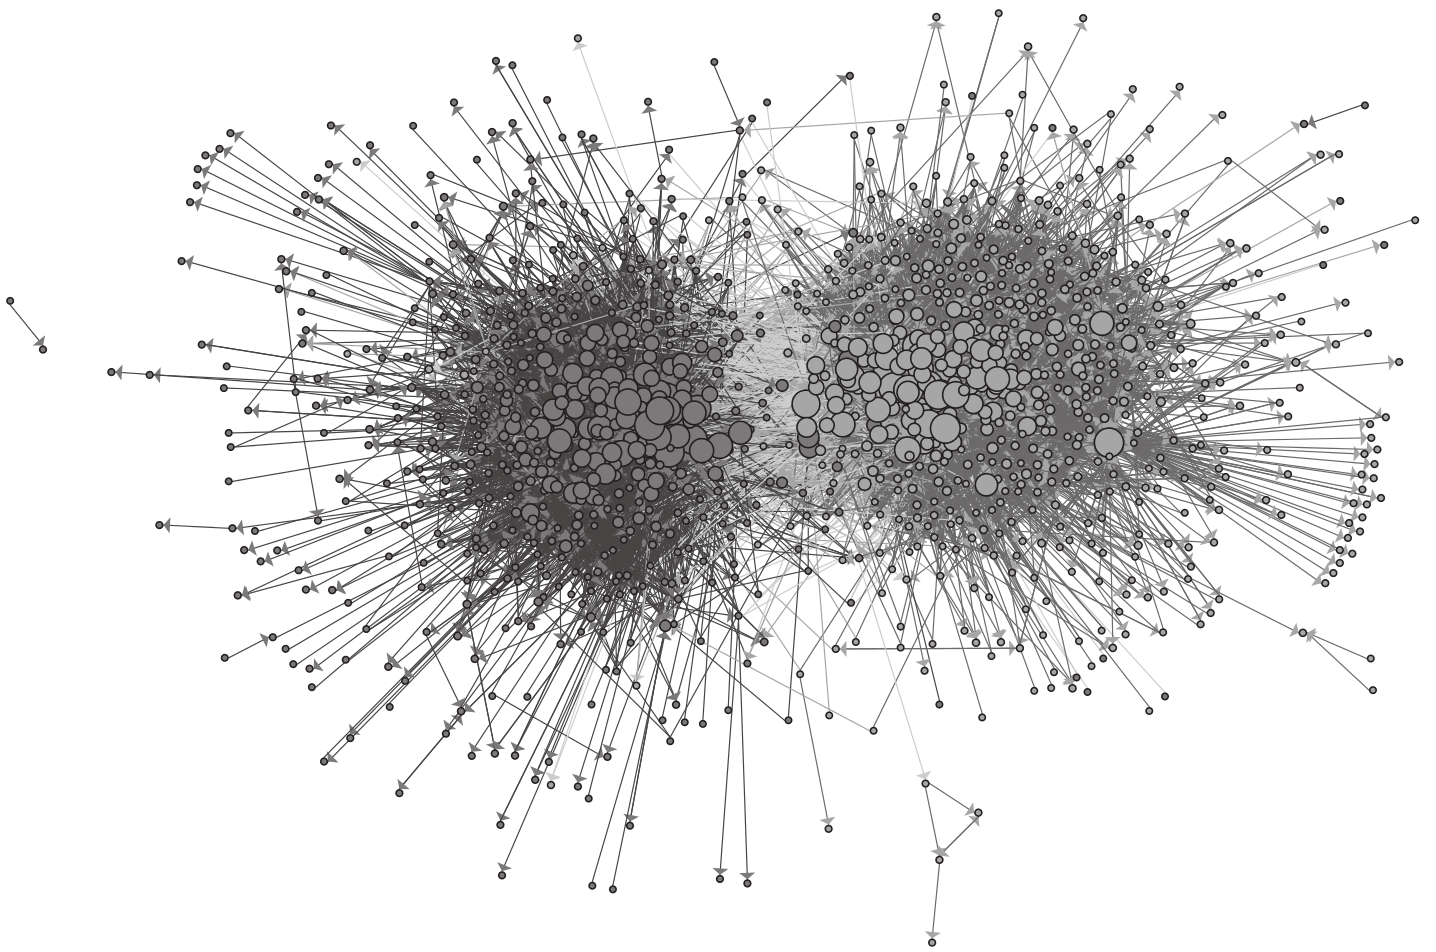
\includegraphics[width=0.8\linewidth]{images/network_structure_of_political_blogs.png}
\end{figure}

Ce sont divers exemples que nous allons essayer d'analyser. Sur Internet, il y a beaucoup de nœuds avec de grandes capacités de calcul et de stockage. Grâce à de nouveaux outils utilisés sur internet pour analyser l'information, on peut observer la structure des graphes (ce qu'on ne pouvait pas faire avant).

\section{Introduction}
\begin{itemize}
\item Structure des réseaux (Facebook, Twitter, réseau économique,...).
\item Comportement des participants (interactions : chaque nœud sera un participant et va interagir).En principe, chaque nœud ne voit que son voisinage et interagit en conséquence.

\begin{itemize}
	\item Interactions \textit{locales} avec conséquences \textit{globales}.
	Il faut faire le lien entre ces deux choses.
	\item Effets non attendus. Par exemple les réseaux routiers : s'il y a des bouchons, on augmente la capacité du réseau (en ajoutant une voie). 
	Le résultat peut être contre intuitif, ça peut être :
	\begin{itemize} 
		\item Une réduction des transferts.
		\item Une augmentation du trafic. (résultat opposé à celui attendu)
	\end{itemize}	
	\item Le \textbf{Paradoxe de Braess} nous dit que l'ajout d'une nouvelle capacité à un réseau peut réduire la performance globale (effet non attendu).
Il faut donc comprendre comment le réseau fonctionne pour prévoir la réaction à une modification plutôt que d'agir impulsivement et avoir des effets non attendus.
\end{itemize}
\end{itemize}

\section{Nouvelle discipline}
Les graphes et leurs propriétés évoluent avec le temps, ce n'est pas statique.

Nouvelles disciplines pour analyser des graphes d'informations tirés de sites comme YouTube, Flicker, etc.

Synthèse de 3 disciplines :
\begin{enumerate}

	\item Mathématiques : théorie des graphes
	\item Mathématiques : théorie des jeux\\
		Exemple : YouTube impose ses règles, c'est le croupier, et ceux qui utilisent YouTube sont des joueurs.
	\item Sociologie : étude des groupes sociaux\\
		les participants sont humains ou guidés par un humain. Il n'est pas uniquement question de mathématiques, il faut aussi comprendre les humains.
\end{enumerate}

Dans ce cours, nous nous concentrerons principalement sur la théorie des graphes. La théorie des jeux sera abordée de façon intuitive, et nous parlerons un peu de la sociologie.

\subsection{Théorie des jeux}
On a un ensemble de participants qui jouent à "un jeu" (un ensemble de règles suivies par tous les participants). Chaque participant doit agir : 

\begin{itemize}
\item Simple à spécifier (comme les échecs : 2 participants et 1 action en alternance). 
\item Compliqué : pas d'alternance, tout le monde agit en même temps. C'est un système concurrent.
\end{itemize}

Exemple d'action simple : la vente aux enchères : 
	nombre fini de participants,
	règles simples et définies (différentes techniques sont possibles)
	
\vspace{1cm}

On va rester intuitif sur ce sujet, mais si on veut être plus précis, il y a des champs mathématiques qui étudient les systèmes concurrents.

Enfin, on peut aussi voir que la position dans le graphe peut aussi apporter des avantages.

\begin{itemize}
	\item \textbf{Figure 1.8} Réseau d'interaction économique entre pays. Structure de l'économie mondiale : Hong Kong a un gros avantage, il a une porte d'entrée vers la Chine (à l'époque). Certains pays sont des partenaires privilégie des États-Unis... 

\begin{figure}[!ht]
\centering
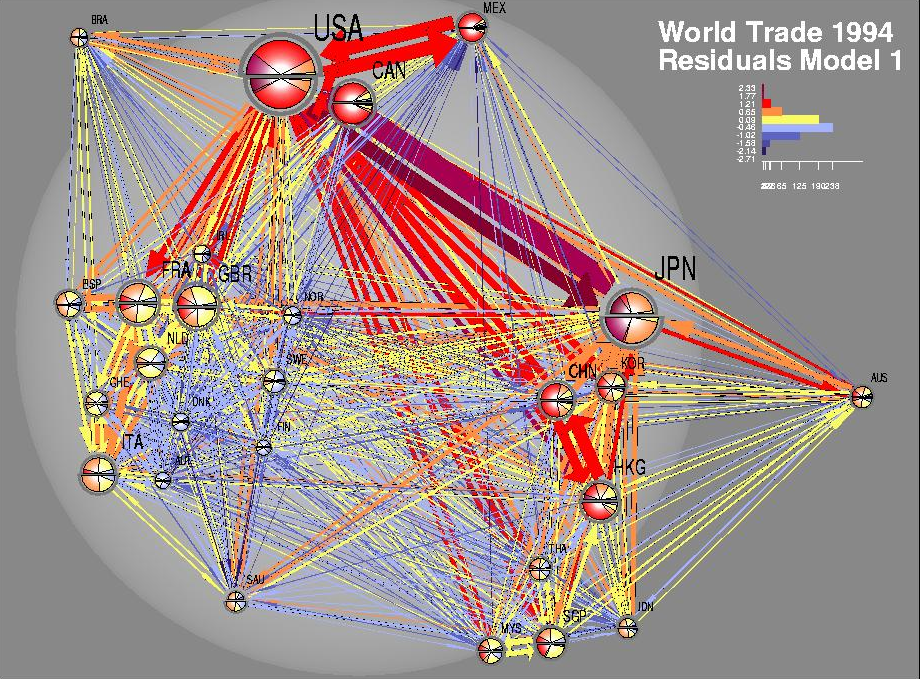
\includegraphics[width=0.8\linewidth]{images/network_international_trade.png}
\end{figure}

	\item \textbf{Figure 1.9} Chemins de commerces médiévaux en Europe. Une position stratégique donne des avantages. Tous ces avantages viennent de la structure du réseau (notons que le comportement d'un participant peut dépendre de la structure).
\begin{figure}[!H]
\centering
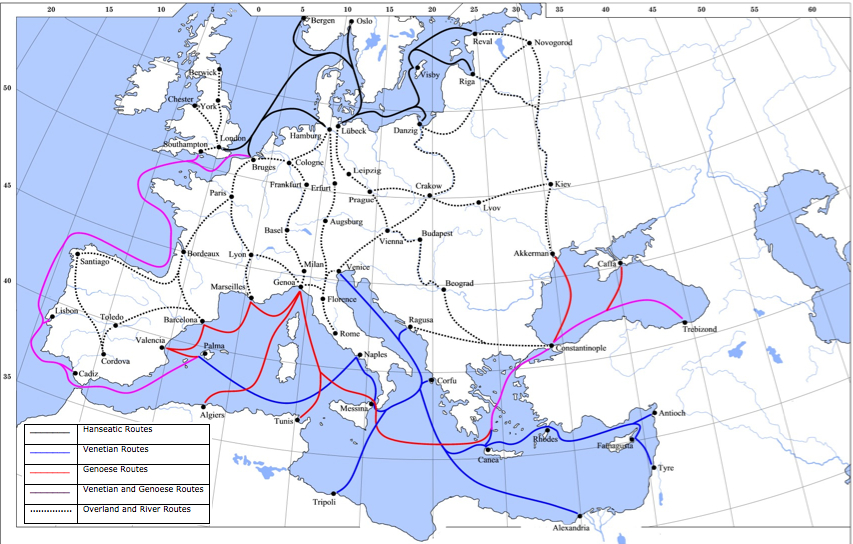
\includegraphics[width=0.9\linewidth]{images/map_of_medieval_trade_routes.png}
\end{figure}
\end{itemize}

Si on observe correctement le réseau, on peut se placer en position d'avantage et se mettre à une position qui donne plus de pouvoir.

Si on connaît la structure, une petite action peut suffire pour arrêter une épidémie en coupant les liens par lesquels cette épidémie pourrait se répandre.
